\chapter{波导}
\label{chap:waveguide}
本章我们研究金属边界下的电磁场,这是一个相当重要且实用的题材。因为
在波长为米量级(或更短)的高频情况下,只有利用线度与波长相当的金属结构才能有效产生和发送电磁波。
% 在更高(红外)频率下,介电光纤在电信行业中被广泛应用。
我们在本章里先考虑在一个导体附近的场,并讨论场对表面的穿透以及伴随的电阻损失。
然后讨论了一般的波导和谐振腔中的电磁波等问题,并进行了具体说明。
用两种不同观点讨论波导中的衰减和谐振腔的$Q$值。
% 其次把地球-电离层系统当作谐振腔处理,接着简短地讨论电介质波导。我们还阐述波导中任意场的简正模展开,并应用到定域源产生的场。本章最后把简正模展开进一步应用到用变分法处理波导中障碍物问题。

\section{导体表面和内部的场}
理想导体(perfect conductor)和超导体(superconductor)的异同?
最大的不同是不存在理想导体,但存在超导体。

\paragraph{理想导体}

% 首先考虑一个法向量n的表面,从一侧的完美导体向外进入另一侧的非导电介质。

由于理想导体内部的电荷会随着场的变化而瞬间移动,故其内部是没有电场的。
其表面电荷密度$\varsigma$ (此处符号与电导率$\sigma$区分)和表面电流密度$\bm\jmath$由理想导体外的法向电位移$\bm D$和切向磁场$\bm H$给出:
\begin{subequations}
    \begin{align}
        \nvec n\cdot\bm D&=\varsigma,\\
        \label{eqn:nxH=j}
        \nvec n\times\bm H&=\bm\jmath.
    \end{align}
\end{subequations}
法向量$\nvec n$指向理想导体外部。其余两个边界条件是关于法向$\bm B$和切向$\bm E$的:
\begin{subequations}
    \begin{align}
        \nvec n\cdot(\bm B-\bm B\c)&=0,\\
        \nvec n\times(\bm E-\bm E\c)&=\bm 0.
    \end{align}
\end{subequations}
下标c表示导体。
由此可见:
在理想导体表面,仅存在法向电场$\bm E$和切向磁场$\bm H$,并且这两个场在理想导体内骤降为0。

\paragraph{良导体}

非理想的良导体的电导率$\sigma$有限,其内部会存在电场,
且振幅随趋肤深度(skin depth)指数衰减:
\begin{equation}
    \delta:=\sqrt{\frac2{\mu\c\omega\sigma}}.
\end{equation}
而Ohm定律$\bm J=\sigma\bm E$说明表面没有电流$\bm\jmath$:
% 边界条件应改为
\[
    \uvec n\times(\bm H-\bm H\c)=\bm 0,
\]
由于场在垂直于表面的方向上的空间变化比平行方向快得多,因此和法向导数相比,切向导数可以忽略。若$\xi$表示导体向内的法向坐标,则
\[
    \nabla\simeq-\uvec n\pp\xi.
\]
忽略导体内的位移电流,谐振场的Maxwell方程变为
\begin{align*}
    \bm E\c&\simeq\frac1\sigma\curl\bm H\c\simeq-\frac1\sigma\uvec n\times\pv{\bm H\c}\xi,\\
    \bm H\c&=-\i\frac1{\mu\c\omega}\curl\bm E\c\simeq\i\frac1{\mu\c\omega}\uvec n\times\pv{\bm E\c}\xi.
\end{align*}
变形得到
\begin{align*}
    \Bigkh{\pp[2]\xi+\i\frac2{\delta^2}}(\uvec n\times\bm H\c)&\simeq\bm 0,\\
    \uvec n\cdot\bm H\c&\simeq 0.
\end{align*}
第二个方程说明:导体内$\bm H$平行于表面,这与边界条件相符。解得
\begin{equation}
    \bm H\c=\bm H_\parallel\e{-\xi/\delta}\e{\i\xi/\delta}.
\end{equation}
$\bm H_\parallel$是导体外表面的切向磁场,则导体内电场
\begin{equation}
    \bm E\c\simeq\sqrt{\frac{\mu\c\omega}{2\sigma}}(1-\i)(\uvec n\times\bm H_\parallel)\e{-\xi/\delta}\e{\i\xi/\delta}.
\end{equation}
故导体内的$\bm H\c$和$\bm E\c$与表面平行,大小随指数迅速衰减,二者有相位差,且磁场比电场强得多。
在表面外侧,除了法向的$\bm E$和切向的$\bm H$外,还有$\bm E$的一个微小的切向分量存在。
这意味着有功率流入导体,每单位面积吸收功率的时间平均为
\begin{equation}
    \dv{P_\text{loss}}a=-\frac12\Re[\uvec n\cdot(\bm E\times\bm H\cj)]=\frac{\mu\c\omega\delta}4|\bm H_\parallel|^2.
\end{equation}
可把这个结果简单地解释为导体内的Ohm损失。
每单位体积内Ohm损失率的时间平均为
% 由Ohm定律,导体表面附件有电流密度$\bm J=\sigma\bm E\c$,而
\[
    \dv{P_\text{loss}}V=\frac12\bm J\cdot\bm E\cj=\frac\sigma 2|\bm J|^2.
\]
由于电流密度$\bm J$局限于导体表面下的薄层内,
其等效有效面电流密度为
\begin{equation}
    \label{eqn:jeff}
    \bm\jmath\eff:=\int\zti\bm J\d\xi=\uvec n\times\bm H_\parallel.
\end{equation}
其形式与理想导体\eqref{eqn:nxH=j}相同,
只是理想面电流密度$\bm\jmath$换成了等效面电流密度$\bm\jmath\eff$。
功率损失可以用等效面电流密度表示:
\begin{equation}
    \label{eqn:dPloss/da}
    \dv{P_\text{loss}}a=\frac1{2\sigma\delta}|\bm\jmath\eff|^2.
\end{equation}
可定义等效表面电阻$R_\text s=1/\sigma\delta$。
% 这说明$1/2\sigma\delta$起着导体表面电阻的作用。
因此,只要我们解出理想导体边界的场,就可以通过\eqref{eqn:jeff}和\eqref{eqn:dPloss/da}给出的$\bm\jmath\eff$近似地算出实际波导、谐振腔和传输线的电阻损失。

\section{柱形波导和谐振腔}

本章研究电磁波在中空金属柱体内的传播和激发。
如果柱体具有端面,就叫做谐振腔(cavity),否则就叫做波导(waveguide)。
本节考虑理想导体作为边界面,在实际应用中发生的能量损失,可用上一节的方法来估计。

柱体内是介电常数$\varepsilon$、磁导率$\mu$的均匀非耗散介质。
当柱体内的场具有谐振关系$\e{-\i\omega t}$时,Maxwell方程组可化为以下形式:
\begin{subequations}
    \begin{align}
        \div\bm E&=0,\\
        \div\bm B&=0,\\
        \curl\bm E&=\i\omega\bm B,\\
        \curl\bm B&=-\i\mu\varepsilon\omega\bm E.
    \end{align}
\end{subequations}
得到Helmholtz方程:
\[
    (\lapla+\mu\varepsilon\omega^2)\bm E=\bm 0,
\]
假定柱形曲面$S$的截面形状和大小沿轴不变,称轴线方向为纵向(longitudinal),垂直于纵向的方向为横向(transverse)。
由边界限制,单独考虑纵向($z$轴)的空间变化:
\[
    \bm E(x,y,z,t)=\bm E(x,y)\e{\i(\pm k_zz-\omega t)},
\]
通过线性组合可以给出纵向的行波或驻波。
目前,纵向波数$k_z$是一个未知参数,它可能是实数也可能是复数。
假定了场对$z$有上述依赖关系后,波动方程就简化为二维形式:
\begin{equation}
    \label{eqn:lapla_tE}
    (\lapla_\t+\mu\varepsilon\omega^2-k_z^2)\bm E=0,
\end{equation}
其中$\lapla_\t$表示Laplace算符的横向部分:
\[
    \lapla=:\lapla_\t+\pp[2]z,
\]
将场分解为横向和纵向两个分量$\bm E=\bm E_\t+\bm E_z$,有
\begin{subequations}
    \begin{align}
        \bm E_\t&=(\uvec z\times\bm E)\times\uvec z,\\
        \bm E_z&=E_z\uvec z,
    \end{align}
\end{subequations}
Maxwell方程组变为
\begin{subequations}
    \label{eqn:EtEzBtBz}
    \begin{align}
        \nabla_\t\cdot\bm E_\t+\pv{E_z}z&=0,\\
        \nabla_\t\cdot\bm B_\t+\pv{B_z}z&=0,\\
        \nabla_\t E_z-\pv{\bm E_\t}z&=\i\omega\uvec z\times\bm B_\t,\\
        \uvec z\cdot(\nabla_\t\times\bm E_\t)&=\i\omega\bm B_z,\\
        \nabla_\t B_z-\pv{\bm B_\t}z&=-\i\mu\varepsilon\omega\uvec z\times\bm E_\t,\\
        \uvec z\cdot(\nabla_\t\times\bm B_\t)&=\i\mu\varepsilon\omega\bm E_z.
    \end{align}
\end{subequations}
结合纵向波数的关系式\eqref{eqn:lapla_tE},$\bm E_\t,\bm B_\t$可以被$E_z,B_z$确定
\begin{subequations}
    \label{eqn:EtBt=EzBz}
    \begin{align}
        \label{eqn:Et=EzBz}
        \bm E_\t&=\i\frac1{\mu\varepsilon\omega^2-k_z^2}(k_z\nabla_\t E_z-\omega\uvec z\times\nabla_\t B_z),\\
        \label{eqn:Bt=EzBz}
        \bm B_\t&=\i\frac1{\mu\varepsilon\omega^2-k_z^2}(k_z\nabla_\t B_z+\mu\varepsilon\omega\uvec z\times\nabla_\t E_z),
    \end{align}
\end{subequations}

\paragraph{TEM模式}

在讨论中空柱体内可以存在的各种场之前,我们先介绍简并型或特殊型解:横电磁(transverse electromagnetic, TEM)波。这种解只有垂直于传播方向的横场分量,$E_z=B_z=0$且
\begin{subequations}
    \begin{align}
        \nabla_\t\cdot\bm E_\text{TEM}&=0,\\
        \nabla_\t\times\bm E_\text{TEM}&=\bm 0,
    \end{align}
\end{subequations}
因此$\bm E_\text{TEM}$是二维静电问题的一个解。纵向波数就是无限介质中的波数
\begin{equation}
    \label{eqn:TEM k0}
    k_z=k_0:=\omega\sqrt{\mu\varepsilon},
\end{equation}
磁场 
\[
    \bm B_\text{TEM}=\pm\sqrt{\mu\varepsilon}\uvec z\times\bm E_\text{TEM},
\]
电导率为无穷大的单个中空柱形导体内不可能存在TEM模。为了运载TEM模,必须有两个及以上的等势面(比如同轴线)。TEM模的一个重要性质是不存在截止频率,即任意$\omega$均可以传播($k_z$均是实数)。
\paragraph{TE模式和TM模式}
横电(TE)波和横磁(TM)波是在中空柱体内(以及高频时的传输线上)出现两类场的构型,
可以通过纵向分量$E_z$和$B_z$满足的波动方程以及边界条件得到。
对于理想导电柱体,边界上电场为法向,磁场为切向:
\begin{subequations}
    \begin{align}
        \uvec n\times\bm E&=\bm0,\\
        \uvec n\cdot\bm B&=0,
    \end{align}
\end{subequations}
% 对于给定频率$\omega$,波数$k$只可能是特定值(波导情况);或对于给定波数$k$,频率$\omega$只能是特定值(谐振腔)。
由于$E_z$和$B_z$边界条件不同,所以本征值一般是不同的,场自然可分为两种模式:
\begin{compactitem}
	\item TM模式:磁场为横向($B_z=0$),边界条件:
    \begin{equation}
        E_z|_S=0;
    \end{equation}
	\item TE模式:电场为横向($E_z=0$),边界条件:
    \begin{equation}
        \edg{\pv{B_z}n}_S=0,
    \end{equation}
\end{compactitem}
\section{波导}
% 当波在一个均匀截面的中空波导中传播时,可得
由\eqref{eqn:EtEzBtBz},
TM波和TE波的横磁场和横电场的关系如下:
\[
    \bm H_\t=\pm\uvec z\times\frac{\bm E_\t}Z,
\]
式中$Z$定义为波阻抗(wave impedance):
\[
    Z:=\begin{cases}
        \frac{k_z}{\varepsilon\omega}=\frac{k_z}{k_0}\sqrt{\frac\mu\varepsilon},&\text{TM}\\
        \frac{\mu\omega}{k_z}=\frac{k_0}{k_z}\sqrt{\frac\mu\varepsilon},&\text{TE}
    \end{cases}
\]
这里$k_0$由\eqref{eqn:TEM k0}给出。
特别地,自由空间阻抗(impedance of free space)为
\begin{equation}
    Z_0=\sqrt{\frac{\mu_0}{\varepsilon_0}}=\mu_0c\simeq 120\pi\,\si{\ohm}
\end{equation}
横向场可由纵向场决定
\begin{subequations}
    \label{eqn:TE/TM field psi}
    \begin{alignat}{2}
        \label{eqn:TM field psi}
        \text{TM}&:\quad&\bm E_\t&=\pm\i\frac{k_z}{k\c^2}\nabla_\t\psi,\quad E_z=\psi\e{\pm\i k_zz};\\
        \label{eqn:TE field psi}
        \text{TE}&:\quad&\bm H_\t&=\pm\i\frac{k_z}{k\c^2}\nabla_\t\psi,\quad H_z=\psi\e{\pm\i k_zz}.
    \end{alignat}
\end{subequations}
其中$k\c^2=\mu\varepsilon\omega^2-k_z^2$。
标量函数$\psi$满足二维波动方程
\begin{equation}
    \label{eqn:laplat+kc2}
    (\lapla_\t+k\c^2)\psi=0,
\end{equation}
根据边界条件:
\begin{alignat*}{2}
    \text{TM}&:&\psi|_S&=0;\\
    \text{TE}&:&\quad\edg{\pv\psi n}_S&=0.
\end{alignat*}
可以确定一系列本征值$k_{\mathrm ci}$和本征函数$\psi_i$,这些不同的解称为波导的模式(mode)。
\begin{definition}
    {截止频率}{cutoff frequency}
    定义单个模式的截止频率(cutoff frequency):
    \begin{equation}
        \label{eqn:cutoff omega}
        \omega\c:=\frac{k\c}{\sqrt{\mu\varepsilon}},
    \end{equation}
    相应的波长$\lambda\c$称为截止波长。
\end{definition}
对于给定的频率$\omega$,单个模式对应的波数
\begin{equation}
    k_z=\sqrt{\mu\varepsilon}\sqrt{\omega^2-\omega\c^2}.
\end{equation}
截止频率的意义为:
\begin{compactitem}
    \item 当$\omega>\omega\c$时,$k_z^2>0$,模式可以在波导中传播;
    \item 当$\omega<\omega\c$时,$k_z^2<0$,模式不能在波导中传播。
\end{compactitem}
因此给定频率上,只有有限个模式可以传播。
可以通过选择波导的尺寸,使得在使用频率上只能出现最低模式的波。

\paragraph{色散关系}

均匀介质波导中的波数$k_z$总是小于无限空间中的波数$k_0$,因此相速度$v_\varphi$大于无限空间中的光速:
\[
    v_\varphi=\frac\omega{k_z}=\frac1{\sqrt{\mu\varepsilon}}\frac1{\sqrt{1-(\omega\c/\omega)^2}}>\frac1{\sqrt{\mu\varepsilon}}.
\]
而群速度小于光速,并且在介质频率处为0:
\[
    v_\text g=\dv\omega{k_z}=\frac1{\sqrt{\mu\varepsilon}}\sqrt{1-\Bigkh{\frac{\omega\c}\omega}^2}<\frac1{\sqrt{\mu\varepsilon}}.
\]
因此并不违反相对论,并且有关系
\begin{equation}
    v_\varphi v_\text g=\frac1{\mu\varepsilon}.
\end{equation}
$\omega\vs k_z$的关系称为色散曲线,曲线上的点的幅角是相速度,切线斜率是群速度。
在均匀传输系统中是双曲线。

\subsection{矩形波导}
\label{ssec:rectangular waveguide}

在内尺寸为$a,b$的矩形波导中(不失一般性取$a>b$),
如\figref{fig:rectangle waveguide} 所示:
\begin{center}
    \includegraphics[page=27]{figures/tikz/layouts.pdf}
    \captionof{figure}{矩形波导}
    \label{fig:rectangle waveguide}
\end{center}
采用直角坐标,
波动方程\eqref{eqn:laplat+kc2}为:
\begin{equation}
    \Bigkh{\pp[2]x+\pp[2]y+k\c^2}\psi=0,
\end{equation}
分离变量$\psi(x,y)=X(x)Y(y)$可得
\begin{align*}
    X(x)&=A\cos(k_xx)+B\sin(k_xx),\\
    Y(y)&=C\cos(k_yy)+D\sin(k_yy).
\end{align*}
满足$k\c^2=k_x^2+k_y^2$,故
\begin{equation}
    k_x^2+k_y^2+k_z^2=k_0^2=\mu\varepsilon\omega^2.
\end{equation}

\paragraph{TE模式}

$E_z=0,\,H_z=\psi$,边界上$\p\psi/\p n=0$可得
\begin{equation}
    \psi_{mn}=A\cos(k_xx)\cos(k_yy),\quad k_x=\frac{m\pi}a,\;k_y=\frac{n\pi}b.
\end{equation}
截止频率为
\begin{equation}
    \omega_{mn}=\frac\pi{\sqrt{\mu\varepsilon}}\sqrt{\Bigkh{\frac ma}^2+\Bigkh{\frac nb}^2}.
\end{equation}
其中$m,n$不同时为0,则TE模式的最低截止频率为TE$_{10}$,对应的
\[
    \omega_{10}=\frac\pi{\sqrt{\mu\varepsilon}a},\quad\lambda_{10}=2a\frac{\sqrt{\mu\varepsilon}}c.
\]
% 在自由空间(即波导中没有介质)中正好$\lambda_{10}=2a$。
由\eqref{eqn:TE field psi}和\eqref{eqn:Et=EzBz},场的表达式为:
\begin{subequations}
    \begin{align}
        H_x&=-\i\frac{k_zk_x}{k\c^2}H_0\sin(k_xx)\cos(k_yy)\e{\i(k_zz-\omega t)},\\
        H_y&=-\i\frac{k_zk_y}{k\c^2}H_0\cos(k_xx)\sin(k_yy)\e{\i(k_zz-\omega t)},\\
        H_z&=H_0\cos(k_xx)\cos(k_yy)\e{\i(k_zz-\omega t)},\\
        E_x&=-\i\frac{\omega\mu k_y}{k\c^2}H_0\cos(k_xx)\sin(k_yy)\e{\i(k_zz-\omega t)},\\
        E_y&=\i\frac{\omega\mu k_x}{k\c^2}H_0\sin(k_xx)\cos(k_yy)\e{\i(k_zz-\omega t)},\\
        E_z&=0.
    \end{align}
\end{subequations}
虚数单位$\i$说明传播方向上$\bm H_\t,\bm E_\t$与$H_z$有$90\degree$的相位差。

由此便可画出不同TE模式的电场线和磁场线。如\figref{fig:waveguide rect TE} 所示为$xy$截面,蓝色实线是电场线、红色虚线是磁场线(的投影)。
注意磁场线不接触内壁,而是会在$z$方向延伸形成回路。
\begin{center}
    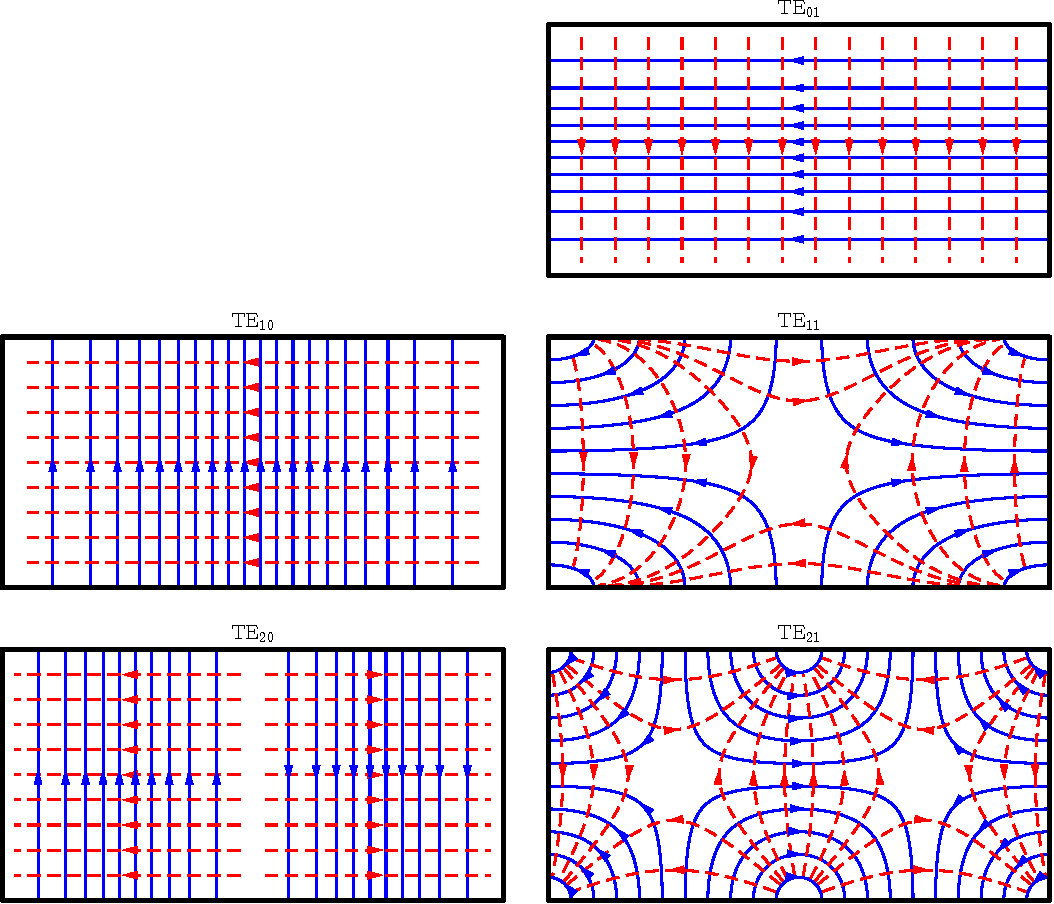
\includegraphics[width=0.8\linewidth]{figures/waveguide_rect_TE.pdf}
    \captionof{figure}{矩形波导的前几个TE模式}
    \label{fig:waveguide rect TE}
\end{center}
可见,TE$_{m0}$模式就是TE$_{10}$模式在$x$方向上复制$m$倍。
同样地,
TE$_{0n}$模式就是TE$_{01}$模式在$y$方向上复制$n$倍;
TE$_{mn}$模式就是TE$_{11}$模式$x$方向上复制$m$倍、在$y$方向上复制$n$倍。

\paragraph{TM模式}
$H_z=0,\,E_z=\psi$,边界上$\psi=0$可得
\begin{equation}
    \psi_{mn}=A\sin(k_xx)\sin(k_yy),\quad k_x=\frac{m\pi}a,\;k_y=\frac{n\pi}b.
\end{equation}
截止频率表达式同TM模,但由于$\psi\not\equiv 0$,故$m,n$均不能为0,最低模式为TM$_{11}$。
\begin{subequations}
    \begin{align}
        H_x&=-\i\frac{\omega\varepsilon k_y}{k\c^2}E_0\sin(k_xx)\cos(k_yy)\e{\i(k_zz-\omega t)},\\
        H_y&=\i\frac{\omega\varepsilon k_x}{k\c^2}E_0\cos(k_xx)\sin(k_yy)\e{\i(k_zz-\omega t)},\\
        H_z&=0,\\
        E_x&=\i\frac{k_zk_x}{k\c^2}E_0\cos(k_xx)\sin(k_yy)\e{\i(k_zz-\omega t)},\\
        E_y&=\i\frac{k_zk_y}{k\c^2}E_0\sin(k_xx)\cos(k_yy)\e{\i(k_zz-\omega t)},\\
        E_z&=E_0\sin(k_xx)\sin(k_yy)\e{\i(k_zz-\omega t)}.
    \end{align}
\end{subequations}
同样地可以画出TM模式在截面上的电场线和磁场线,由于TM$_{mn}$模式同样只是TM$_{11}$模式的简单复制,故只需画出TM$_{11}$模式,如\figref{fig:waveguide rect TM} 所示:
\begin{center}
    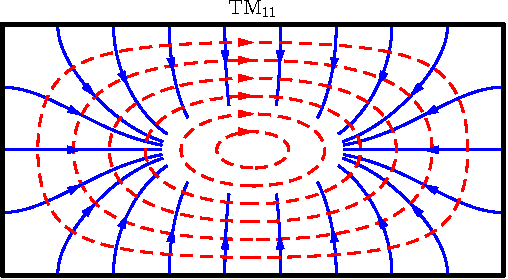
\includegraphics[width=0.4\linewidth]{figures/waveguide_rect_TM.pdf}
    \captionof{figure}{矩形波导的TM$_{11}$模式}
    \label{fig:waveguide rect TM}
\end{center}

\paragraph{传输特性}

根据截止频率的表达式,TE$_{10}$模式具有最低的截止频率。一般波导内为真空,相应的截止波长$\lambda_{10}=2a$。其次为TE$_{20}$或TE$_{01}$。理论上当
\[
    \max(a,2b)\leq\lambda<2a
\]
时,波导内只存在TE$_{10}$模式,而其余频率均被截止。因此通常矩形波导会被设计成$a=2b$,且尺寸随着工作频率的增加而减小。

\subsection{圆波导}

在内径为$a$的圆形波导中,
\begin{center}
    \includegraphics[page=28]{figures/tikz/layouts.pdf}
    \captionof{figure}{圆波导}
    \label{fig:circle waveguide}
\end{center}
采用柱坐标,波动方程\eqref{eqn:laplat+kc2}为:
\begin{equation}
    \Bigkh{\pp[2]\rho+\frac1\rho\pp\rho+\frac1{\rho^2}\pp[2]\phi+k\c^2}\psi=0,
\end{equation}
分离变量$\psi(\rho,\phi)=R(\rho)\Phi(\phi)$可得
\begin{align*}
    R(\rho)&=AJ_m(k\c\rho)+BN_m(k\c\rho),\\
    \Phi(\phi)&=\e{\pm\i m\phi}.
\end{align*}
其中$J_m,N_m$分别是第一、二类Bessel函数,由$R(0)<\infty$知$B=0$。由于极轴的选取是任意的,取$D=0$。

\paragraph{TM模式}

$H_z=0,\,E_z=\psi$,边界上$\psi=0$可得
\begin{equation}
    \psi_{mn}=AJ_m(k\c\rho)\e{\pm\i m\phi},\quad k\c=\frac{x_{mn}}a.
\end{equation}
其中$x_{mn}$表示$J_m$的第$n$个正零点。
场的表达式为
\begin{subequations}
    \begin{align*}
        H_\rho&=\pm m\frac{\omega\varepsilon k_z}{k\c^2\rho}E_0J_m(k\c\rho)\e{\i(k_zz-\omega t\pm m\phi)},\\
        H_\phi&=\i\frac{\omega\varepsilon k_z}{k\c}E_0J_m'(k\c\rho)\e{\i(k_zz-\omega t\pm m\phi)},\\
        H_z&=0,\\
        E_\rho&=\i\frac{k_z}{k\c}E_0J_m'(k\c\rho)\e{\i(k_zz-\omega t\pm m\phi)},\\
        E_\phi&=\mp m\frac{k_z}{k\c^2\rho}E_0J_m(k\c\rho)\e{\i(k_zz-\omega t\pm m\phi)},\\
        E_z&=E_0J_m(k\c\rho)\e{\i(k_zz-\omega t\pm m\phi)}.
    \end{align*}
\end{subequations}

\paragraph{TE模式}

$E_z=0,\,H_z=\psi$,边界上$\p\psi/\p n=0$可得
\begin{equation}
    \psi_{mn}=AJ_m(k\c\rho)\e{\pm\i m\phi},\quad k\c=\frac{x_{mn}'}a.
\end{equation}
其中$x_{mn}'$表示$J_m'$的第$n$个正零点。
场的表达式为
\begin{subequations}
    \begin{align*}
        H_\rho&=\i\frac{k_z}{k\c}H_0J_m'(k\c\rho)\e{\i(k_zz-\omega t\pm m\phi)},\\
        H_\phi&=\mp m\frac{k_z}{k\c^2\rho}H_0J_m(k\c\rho)\e{\i(k_zz-\omega t\pm m\phi)},\\
        H_z&=H_0J_m(k\c\rho)\e{\i(k_zz-\omega t\pm m\phi)},\\
        E_\rho&=\pm m\frac{\omega\mu k_z}{k\c^2\rho}H_0J_m(k\c\rho)\e{\i(k_zz-\omega t\pm m\phi)},\\
        E_\phi&=\i\frac{\omega\mu k_z}{k\c}H_0J_m'(k\c\rho)\e{\i(k_zz-\omega t\pm m\phi)},\\
        E_z&=0.
    \end{align*}
\end{subequations}
不难发现,圆波导的TE模式与TM模式场的表达式仅仅是将$E,H$和$\varepsilon,\mu$互换。

\paragraph{前几个$x_{mn}$和$x_{mn}'$分布}

\begin{figure}[H]
    \centering
    \subcaptionbox{$J_m(x)$的零点分布}
        {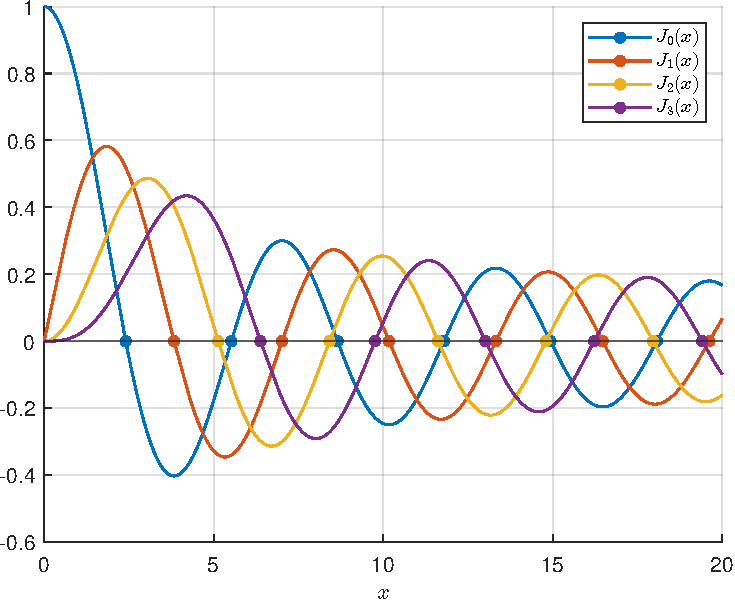
\includegraphics[width=0.45\linewidth]{figures/BesselJzero.pdf}}
    \subcaptionbox{$J_m'(x)$的零点分布}
        {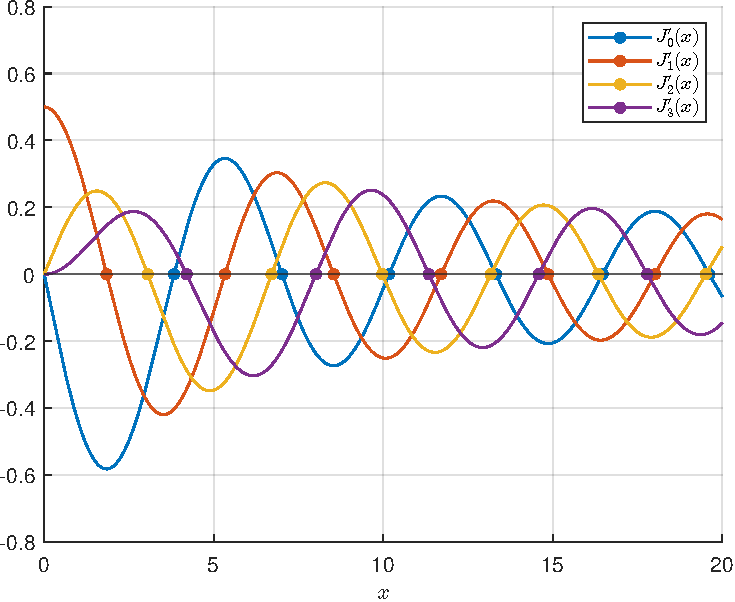
\includegraphics[width=0.45\linewidth]{figures/BesselJpzero.pdf}}
    \caption{$J_m(x)$和$J_m'(x)$的零点分布}
    \label{fig:Bessel function zeros}
\end{figure}

查表知,TE和TM的最低模式分别为TM$_{01}$和TE$_{11}$。
由于$J_0'(x)=-J_1(x)$,TM$_{1n}$和TE$_{0n}$的截止频率相同。

\begin{table}[H]
    \centering
    \caption{$J_m(x)$和$J_m'(x)$的零点}
    \subcaptionbox{$J_m(x)$的零点$x_{mn}$}{
    \begin{tabular}{crrr}
        \toprule
        $x_{mn}$&$n=1$&$n=2$&$n=3$\\
        \midrule
        $m=0$&2.405&5.520&8.654\\
        $m=1$&3.832&7.016&10.173\\
        $m=2$&5.136&8.417&11.620\\
        $m=3$&6.380&9.761&13.015\\
        \bottomrule
    \end{tabular}}
    \quad
    \subcaptionbox{$J_m'(x)$的零点$x_{mn}'$}{
    \begin{tabular}{crrr}
        \toprule
        $x_{mn}'$&$n=1$&$n=2$&$n=3$\\
        \midrule
        $m=0$&3.832&7.016&10.176\\
        $m=1$&1.841&5.331& 8.536\\
        $m=2$&3.054&6.706& 9.970\\
        $m=3$&4.201&8.015&11.346\\
        \bottomrule
    \end{tabular}}
\end{table}


\subsection{介质加载波导}

\paragraph{慢波结构}
带电粒子与电磁波交换能量(加速/减速)要求电磁波的相速度与电子的速度相同。
因此需要波导中的相速度小于等于光速,称为慢波结构。
由于带电粒子在介质中的速度超过介质光速时,会产生Cherenkov辐射,故无法采用全部填充介质的波导。本小节考虑部分填充介质的波导。
\begin{center}
    \includegraphics[page=29]{figures/tikz/layouts.pdf}
    \captionof{figure}{部分填充介质的矩形波导}
    \label{fig:rectangle waveguide part-filled}
\end{center}
% 后面我们将说明不存在TM模式,
考虑TE模式,根据金属边界条件,两部分的场形式为:
\begin{alignat*}{2}
    H_{z1}&=A\cos(k_{x1}x)\cos(k_{y1}y)\e{\i k_zz},&k_{y1}&=\frac{n_1\pi}b,\\
    H_{z2}&=B\cos(k_{x2}(a-x))\cos(k_{y2}y)\e{\i k_zz},&\quad k_{y2}&=\frac{n_2\pi}b.
\end{alignat*}
且
\begin{subequations}
    \begin{align}
        k_{x1}^2+k_{y1}^2+k_z^2=\mu_1\varepsilon_1\omega^2=:k_1^2,\\
        k_{x2}^2+k_{y2}^2+k_z^2=\mu_2\varepsilon_2\omega^2=:k_2^2,
    \end{align}
\end{subequations}
由$H_z$在介质分界$x=d$处连续,可得$n_1=n_2=n$;当$n\neq 0$时,结合
\[
    H_{yi}=\i\frac{k_z}{k_i^2-k_z^2}\pv{H_{zi}}y
\]
在$x=d$处连续,可得$\varepsilon_1\mu_1=\varepsilon_2\mu_2$。即$\varepsilon_1\mu_1\neq\varepsilon_2\mu_2$时,TE$_{mn}$不存在。
% 由$E_y,H_y,H_z$在介质分界$x=d$处连续,可得$n_1=n_2=n$且$n\neq 0$时,
但是TE$_{m0}$可以存在,此时$H_y\equiv 0$,再结合
\[
    E_{yi}=-\i\frac{\omega\mu_i}{k_i^2-k_z^2}\pv{H_{zi}}x
\]
在$x=d$处连续,可得
\begin{equation}
    \frac{\mu_1}{k_{x1}}\tan(k_{x1}d)=\frac{\mu_2}{k_{x2}}\tan(k_{x2}(a-d)),
\end{equation}
再结合
\begin{equation}
    k_{x1}^2-k_{x2}^2=(\mu_1\varepsilon_1-\mu_2\varepsilon_2)\omega^2,
\end{equation}
便可在给定$\omega$下求得$k_{x1},k_{x2}$和$k_z$。
另一方面,也可以令$k_z=0$求得截止频率满足的方程:
\begin{equation}
    \sqrt{\frac{\mu_1}{\varepsilon_1}}\tan(\omega\c\sqrt{\mu_1\varepsilon_1}d)=
    \sqrt{\frac{\mu_2}{\varepsilon_2}}\tan(\omega\c\sqrt{\mu_2\varepsilon_2}(a-d)).
\end{equation}
上式可以通过作图求出交点。显然,TE$_{m0}$的截止频率位于分别完全填充介质1 ($d=a$)和介质2 ($d=0$)的截止频率之间:
\[
    \frac{m\pi}{a\sqrt{\mu_1\varepsilon_1}}<\omega\c<\frac{m\pi}{a\sqrt{\mu_2\varepsilon_2}},
\]

考虑介质2为真空,
当相速度$v_\varphi$等于电子速度(电子在一定能量下速度可以非常接近真空光速)时,即$v_\varphi=\omega/k_z=c$,
有$k_{x2}=0$。

\subsection{波导中的能流和衰减}

我们扩大前面对任意截面形状的柱形波导所作的一般讨论,使它包括沿波导的能流以及波的衰减,后者是当电导率有限时由波导管壁中能量损耗所引起的。我们只限于讨论波导中只存在一种模式的情况;不过将简短提一下简并模式。能流用复Poynting矢量描写;
\begin{equation}
    \bm S=\frac12\bm E\times\bm H\cj=\frac{\omega k}{2\gamma^4}
    \begin{cases}
        \varepsilon\Bigkh{\uvec z|\nabla_\t\psi|^2+\i\frac{\gamma^2}k\psi\nabla_\t\psi\cj},&\text{TM}\\[1ex]
        \mu\Bigkh{\uvec z|\nabla_\t\psi|^2-\i\frac{\gamma^2}k\psi\cj\nabla_\t\psi},&\text{TE}
    \end{cases}
\end{equation}
因为$\psi$一般是实数,\footnote{有可能这样激发一个波导,使得某给定模式或一些模式的线性组合具有复数$\psi$。这时候横向能流对时间的平均值将不为零,但因为它是一个环流,所以实际上只代表贮藏的能量,在实用上不大重要。}
因此$\bm S$的第二项代表无功能流,并且对能流的时间平均没有贡献。总功率流
\[
    P=\int_A\bm S\cdot\uvec z\d a=\frac{\omega k}{2\gamma^4}
    \begin{Bmatrix}
        \varepsilon\\\mu
    \end{Bmatrix}
    \biggkh{\oint_{\p A}\cancel{\psi\cj\pv\psi n}\d\ell-\int_A\psi\cj\nabla_\t^2\psi\d a}.
\]
由特征方程$(\nabla_\t^2+\gamma_\lambda^2)\psi=0$,
\[
    P=\frac1{2\sqrt{\mu\varepsilon}}\biggkh{\frac\omega{\omega_\lambda}}^2\biggkh{1-\frac{\omega_\lambda^2}{\omega^2}}^{1/2}
    \begin{Bmatrix}
        \varepsilon\\\mu
    \end{Bmatrix}
    \int_A\psi\cj\psi\d a.
\]
时间平均能量密度
\[
    u=\frac14\Bigkh{\varepsilon\bm E\cdot\bm E\cj+\frac1\mu\bm B\cdot\bm B\cj},
\]
单位长度的场能量
\[
    U=\frac12\biggkh{\frac\omega{\omega_\lambda}}^2
    \begin{Bmatrix}
        \varepsilon\\\mu
    \end{Bmatrix}
    \int_A\psi\cj\psi\d a,
\]
能流的速度正是群速度
\[
    \frac PU=\frac k\omega\frac1{\mu\varepsilon}=\frac1{\sqrt{\mu\varepsilon}}\sqrt{1-\frac{\omega_\lambda^2}{\omega^2}}=v_\text g.
\]
结合前面说的相速度
\begin{equation}
    v_\text gv_\varphi=\frac1{\mu\varepsilon},
\end{equation}
在无限介质中,$v_\text g$总是小于$v_\varphi$,并且在截止频率时降为零。
\paragraph{良导体的波导}
对于理想导体,$k_\lambda$是实数或纯虚数;而对于电导率有限的良导体来说,$k_\lambda$是一个实数与一个小复数的和。

后面的略。
\paragraph{最小衰减频率}
略。
\section{边界条件的扰动}
略
\section{谐振腔}
一个谐振腔(resonant cavity)可以是任何形状的,具有一个封闭的导体表面。但通常我们将端面放置在一定长度的圆柱形波导上,以产生一个空腔。端面是垂直于圆柱体轴线的平面。

% 由$z=0,d$的边界条件,应有驻波形式:
% \begin{align*}
%     \text{TM}&:&E_z=\psi(x,y)\cos\Bigkh{\frac{p\pi z}d},&&p&=0,1,2,\ldots,\\
%     \text{TE}&:&H_z=\psi(x,y)\sin\Bigkh{\frac{p\pi z}d},&&p&=1,2,3,\ldots,
% \end{align*}
% 特征值频率
% \[
%     \omega_{\lambda_p}^2=\frac1{\mu\varepsilon}\Bigfkh{\gamma_\lambda^2+\Bigkh{\frac{p\pi}d}^2},
% \]

% 对于TM模,$\psi=E_z$,
% \[
%     \psi(\rho,\phi)=E_0J_m(\gamma_{mn}\rho)\e{\pm\i m\phi},\quad\gamma_{mn}=\frac{x_{mn}}R,
% \]
% 其中$x_{mn}$表示$J_m(x)$的第$n$个零点:

% 谐振频率为
% \begin{equation}
%     \omega_{mnp}=\frac1{\sqrt{\mu\varepsilon}}\sqrt{\Bigkh{\frac{x_{mn}}R}^2+\Bigkh{\frac{p\pi}d}^2}.
% \end{equation}

% 对于TE模,$\psi=H_z$,
% \[
%     \gamma_{mn}=\frac{x'_{mn}}R,
% \]
% 其中$x'_{mn}$表示$J'_m(x)$的第$n$个零点:

% 谐振频率为
% \begin{equation}
%     \omega_{mnp}=\frac1{\sqrt{\mu\varepsilon}}\sqrt{\Bigkh{\frac{x'_{mn}}R}^2+\Bigkh{\frac{p\pi}d}^2}.
% \end{equation}
\section{腔内的功率损失}
对于理想导体,$|E(\omega)|$在各个$\omega_i$上是一个个$\delta$函数;而对于良导体,则会有一定的半高宽。

定义品质因子(quality factor)
\begin{equation}
    Q:=\omega_0\frac{\text{stored energy}}{\text{power loss}}.
\end{equation}

